\documentclass[11pt]{amsart}

\usepackage{amsmath,amssymb,amsthm}
\usepackage[margin=1in]{geometry}
\usepackage{mathtools}
\usepackage{booktabs}
\usepackage{tikz}
\usetikzlibrary{arrows.meta,positioning}
\usepackage[colorlinks=true,linkcolor=blue!55!black,citecolor=blue!55!black,urlcolor=blue!55!black]{hyperref}

\theoremstyle{plain}
\newtheorem{theorem}{Theorem}[section]
\newtheorem{proposition}[theorem]{Proposition}
\newtheorem{lemma}[theorem]{Lemma}
\newtheorem{corollary}[theorem]{Corollary}
\theoremstyle{definition}
\newtheorem{definition}[theorem]{Definition}
\newtheorem{example}[theorem]{Example}
\theoremstyle{remark}
\newtheorem{remark}[theorem]{Remark}

% Notation
\newcommand{\Set}{\mathbf{Set}}
\newcommand{\Cat}{\mathbf{Cat}}
\newcommand{\Graph}{\mathbf{Graph}}
\newcommand{\Poly}{\mathrm{Poly}}
\newcommand{\Comon}{\mathrm{Comon}}
\newcommand{\cat}{\mathsf{cat}}
\newcommand{\Ee}{\mathcal{E}}
\newcommand{\sub}{\triangleleft}      % substitution / composition product
\newcommand{\dir}[1]{[#1]}
\newcommand{\sharpc}[1]{#1^{\sharp}}   % the comonoid of an internal category
\newcommand{\id}{\mathrm{id}}
\newcommand{\dom}{\mathrm{dom}}
\newcommand{\cod}{\mathrm{cod}}
\newcommand{\comp}{\mathrm{comp}}
\newcommand{\ob}{\mathrm{ob}}
\DeclareMathOperator{\Mod}{Mod}

\title[Day convolution of polynomial comonoids is the product category, in every topos]
{The Day convolution of two polynomial comonoids is the\\
product internal category --- in every Grothendieck topos}

\author{MacBeth}
\address{Kodamai}
\date{22 October 2026}

\begin{document}

\begin{abstract}
In $\Set$, comonoids for the substitution product $\sub$ of polynomial functors are exactly small
categories, and the Dirichlet (Day-convolution) tensor $\otimes$ of two such comonoids represents
the product category $C\times D$ on the nose. We show this is not an artefact of $\Set$. Let $\Ee$
be any Grothendieck topos and $C,D$ internal categories in $\Ee$, viewed as $\sub$-comonoids
$c,d$ in the category $\Poly(\Ee)$ of internal polynomial functors. Then $c\otimes d$ carries a
canonical comonoid structure whose represented internal category is the product $C\times D$ in
$\Cat(\Ee)$ --- componentwise objects, morphisms, identities and composition --- \emph{on the nose};
and under the internal equivalence $\Comon(\Poly(\Ee),\sub)\simeq\Cat(\Ee)$ the tensor $\otimes$
computes the categorical product. The proof uses only that $\Ee$ is locally cartesian closed and
finitely complete; it never invokes well-pointedness, extensivity, or disjointness of coproducts, so
it is uniform across presheaf and sheaf toposes alike, with $\Set$ as the degenerate case. The
single load-bearing coherence is the distributor $\Sigma(A\times B)\cong(\Sigma A)\times(\Sigma B)$,
which is exactly the local-cartesian-closedness law that Gambino and Kock use to compose polynomial
functors. A worked witness in the presheaf topos $\Graph$, with a loopless object-of-objects carrying
no global element, is machine-checked in Lean.
\end{abstract}

\maketitle

\footnotetext{MacBeth (scotmacbeth) $\cdot$ 2026-10-22 $\cdot$ content commit \texttt{b553b27}.
Theorem~\ref{thm:main-I} (the on-the-nose identification) is proved here. Theorem~\ref{thm:main-II}
(that $\otimes$ is the categorical product) rests on the published internal equivalence of
Shapiro--Spivak \cite{ShapiroSpivak2023}, Thm.~5.6 and Cor.~5.12, and is \emph{not} claimed as a
result of this note. The $\Graph$ witness of \S\ref{sec:graph} is machine-checked
(\texttt{lean/2026-10-21-day-convolution-graph.lean}, Mathlib-free, \texttt{[propext]} only).}

%============================================================
\section{Introduction}
%============================================================

\subsection*{The equivalence chain, and whether it is a feature of \texorpdfstring{$\Set$}{Set}}

A recurring discovery of the last fifteen years is that four superficially different notions of
``directed shape'' coincide:
\[
   \text{containers} \;\simeq\; \text{directed containers} \;\simeq\;
   \text{polynomial comonoids} \;\simeq\; \text{small categories.}
\]
The last of these equivalences is the one this note is about. Write $\Poly$ for the category of
polynomial endofunctors on $\Set$, equipped with the substitution (composition) monoidal product
$\sub$ with unit $y=\mathrm{Id}$. A theorem of Ahman and Uustalu, given its modern comonoid phrasing
by Spivak and collaborators \cite{SGF2021,NiuSpivak2023}, identifies the comonoids in
$(\Poly,\sub,y)$ with small categories:
\[
   \Comon(\Poly,\sub,y) \;\simeq\; \Cat .
\]
A polynomial carries a \emph{second} monoidal product, the Dirichlet tensor $\otimes$, which by
Niu--Spivak \cite[Prop.~3.79]{NiuSpivak2023} is the Day convolution induced on $\Poly$ by the
cartesian structure $(1,\times)$ of $\Set$. The two products interlock into a normal duoidal
structure \cite[Ex.~2.9]{ShapiroSpivak2023}, so $\sub$-comonoids are closed under $\otimes$; and a
short computation (\S\ref{sec:setI}, and \cite[the $\Set$ case]{NiuSpivak2023}) shows that the
resulting comonoid on $c\otimes d$ is precisely the product category $C\times D$.

This is a clean fact about $\Set$. It is natural to ask whether it is \emph{only} a fact about
$\Set$. The question is not idle. The entire value of the equivalence chain, as a foundation for
compositional systems, is that it should be a theorem about \emph{structure}, not about a privileged
ambient universe; and the concrete compositional models one wants --- presheaves on a site of
locations, sheaves on a space of states, graphs of a network --- live in toposes other than $\Set$.
If the Day convolution ceased to be the product category the moment one left $\Set$, the chain would
be a $\Set$-level coincidence rather than a transportable principle.

\subsection*{The main result}

It is not a coincidence. We prove it transports, verbatim, to every Grothendieck topos.

Throughout, $\Ee$ is a Grothendieck topos (equivalently, a left-exact localization of a presheaf
topos); in particular $\Ee$ is locally cartesian closed and finitely complete, and by Gambino--Kock
\cite{GambinoKock2013} the category $\Poly(\Ee)$ of internal polynomial functors exists, carries the
substitution product $\sub$ and the Dirichlet tensor $\otimes$, and its $\sub$-comonoids are internal
categories in $\Ee$. Write $\cat(\Ee):=\Comon(\Poly(\Ee),\sub,y)$. For an internal category $C$ in
$\Ee$ we write $\sharpc{C}\in\cat(\Ee)$ for the corresponding comonoid.

\begin{theorem}[On-the-nose identification]\label{thm:main-I}
Let $C,D$ be internal categories in a Grothendieck topos $\Ee$, with comonoids $c,d\in\cat(\Ee)$.
Then $c\otimes d$ carries a canonical $(\sub,y)$-comonoid structure --- counit $\varepsilon_c\otimes
\varepsilon_d$, comultiplication $\iota\circ(\delta_c\otimes\delta_d)$ via the normal-duoidal
interchanger $\iota$ --- and the internal category it represents is the product internal category
$C\times D$, \emph{on the nose}: object-of-objects $C_0\times D_0$, object-of-morphisms
$C_1\times D_1$, with domain, codomain, identities and composition all componentwise. In symbols,
$c\otimes d=\sharpc{(C\times D)}$ in $\cat(\Ee)$.
\end{theorem}

\begin{theorem}[Universal property]\label{thm:main-II}
Under the internal equivalence $\cat(\Ee)\simeq\Cat(\Ee)$, the Dirichlet tensor $\otimes$ computes the
categorical product in $\cat(\Ee)$, with projections $\pi_C=\id_c\otimes\varepsilon_d$ and
$\pi_D=\varepsilon_c\otimes\id_d$ --- even though $\otimes$, as a monoidal structure on all of
$\Poly(\Ee)$, is \emph{not} the cartesian product.
\end{theorem}

We are careful about what is ours. Theorem~\ref{thm:main-I} is proved here, modulo the two published
facts recalled in \S\ref{sec:prelim} (that $\Poly(\Ee)$ exists over an LCCC, Gambino--Kock
\cite{GambinoKock2013}; and that the duoidal interchanger exists, Shapiro--Spivak
\cite{ShapiroSpivak2023}). Theorem~\ref{thm:main-II} additionally requires the \emph{full} internal
equivalence $\cat(\Ee)\simeq\Cat(\Ee)$ --- including essential surjectivity, to quantify the product's
universal property over \emph{all} comonoids --- which is the published theorem of Shapiro--Spivak
\cite[Thm.~5.6, Cor.~5.12]{ShapiroSpivak2023}. Theorem~\ref{thm:main-II} is therefore a corollary of
their equivalence, not a result of this note; we state it to complete the picture.

\subsection*{Why ``on the nose'', and what the proof does not use}

The phrase ``on the nose'' is doing real work. There is no coherence isomorphism to chase: the
structure maps of $c\otimes d$ --- read off through the comonoid-to-category dictionary --- are
\emph{equal}, as morphisms of $\Ee$, to the structure maps of $C\times D$. The reason is a clean
division of labour. The non-trivial, non-pointwise ingredient of the substitution product $\sub$
(it uses the dependent product $\Pi$, hence an internal hom, hence a Yoneda/Kan formula --- it is
\emph{not} computed objectwise in a presheaf topos) is absorbed entirely into the
comonoid-to-category translation and never resurfaces. What remains, once one is speaking the language
of internal-category data $(C_0,C_1,\dom,\cod,\id,\comp)$, is componentwise finite limits.

Three ingredients the reader might expect to see are conspicuously absent, and their absence is the
sharpening we offer over the folklore ``locally cartesian closed and extensive'' hypothesis:

\begin{itemize}
\item \emph{No well-pointedness.} The counit $\varepsilon_c:c\to y$, which in the $\Set$ picture
``picks the identity $\id_i$ in each hom-set'', is here literally the single identity-assigning
section $\id:C_0\to C_1$ of $\Ee$ --- not a choice of global elements. This is the point at which
every naive $\Set$-level argument would break, and it does not break. The $\Graph$ witness of
\S\ref{sec:graph} is built with a \emph{loopless} object-of-objects, which has no global element at
all, precisely to exhibit this.
\item \emph{No extensivity, no disjointness of coproducts.} The one coherence the comultiplication
needs is the distributor
\(
  \Sigma_{(i,k)}(A_i\times B_k)\;\cong\;(\Sigma_i A_i)\times(\Sigma_k B_k),
\)
and this is \emph{not} a separate extensivity axiom: it is the distributivity of products over
dependent sums that holds in every LCCC --- indeed it is the very law Gambino and Kock invoke to prove
that polynomial functors compose \cite{GambinoKock2013}. Universal coproducts come for free (each
pullback functor $f^\ast$ is a left adjoint, hence preserves colimits).
\item \emph{No cartesianness, and no symmetry of the tensor} for the identification itself.
Symmetry of $\times$ in $\Ee$ is used only to make $\otimes$ symmetric, whose braiding corresponds to
the swap $C\times D\cong D\times C$ --- an addendum, not a hypothesis of Theorem~\ref{thm:main-I}.
\end{itemize}

So the honest reach of the method is ``locally cartesian closed, with the dependent sums that
Gambino--Kock polynomials require'', of which Grothendieck toposes are the canonical --- and
completely general-purpose --- instance. We state the theorems over Grothendieck toposes because they
have everything with no fuss, and flag the maximal-generality form as an open bound in
\S\ref{sec:discussion}.

\subsection*{A question that inverted into its own answer}

This note is the positive residue of a negative-looking investigation. For some months the program
pursued a ``which base $V$?'' question: over which monoidal bases does the Day-convolution-is-product
phenomenon survive? The characteristic failure case was $V=\mathbf{Vec}$. The enriched-category
literature points the same way from a different direction: Lucyshyn-Wright's study of graded and
bigraded categories \cite{LucyshynWright2025} finds that Day-convolution \emph{closure} is special to
$\Set$-like bases and does not transport to a general enriched base $V$ (the paper is about enrichment,
not polynomial comonoids, so this is a parallel signal rather than the same theorem). Read under
``for \emph{all} $V$?'', such findings look like a dead end. Read under ``for \emph{which} $V$?'',
they are the answer: the Day-convolution story is base-sensitive, and asks for a base with genuine
dependent-type structure. The present theorems supply such a base in the cleanest way --- a
Grothendieck topos --- and state the positive side: the product-is-Day-convolution fact does not
merely survive the passage to a topos, it is \emph{uniform} across all of them. They also relocate the
$\mathbf{Vec}$ obstruction precisely: $\mathbf{Vec}$ is not locally cartesian closed, so
$\Poly(\mathbf{Vec})$ and its $\sub$ have no standard construction; the obstruction was never about
cartesianness of the tensor (consistent with $\mathbf{Vec}$'s $\otimes$ distributing happily over
$\oplus$).

\subsection*{Outline} \S\ref{sec:prelim} recalls $\Poly(\Ee)$, the two products, the
comonoid--category dictionary, and the interchanger, over a general LCCC base. \S\ref{sec:setI} proves
Theorem~\ref{thm:main-I} in three steps: the underlying object (finite limits), the interchanger's
distributor (the LCCC law), and the structure trace. \S\ref{sec:product} records
Theorem~\ref{thm:main-II} as a corollary of the Shapiro--Spivak equivalence. \S\ref{sec:transport}
isolates, in a table, exactly what the base must supply. \S\ref{sec:graph} gives the machine-checked
$\Graph$ witness. \S\ref{sec:discussion} states the honest open bounds.

%============================================================
\section{Preliminaries}\label{sec:prelim}
%============================================================

We fix a Grothendieck topos $\Ee$; the only properties used are that $\Ee$ is locally cartesian closed
(LCCC) and finitely complete, so the reader may equally read ``LCCC with Gambino--Kock polynomials''
throughout. Recall that LCCC means each slice $\Ee/I$ is cartesian closed; equivalently each pullback
functor $f^\ast:\Ee/J\to\Ee/I$ along $f:I\to J$ has a right adjoint $\Pi_f$ (dependent product), in
addition to its left adjoint $\Sigma_f$ (dependent sum). We freely use the adjoint string
$\Sigma_f\dashv f^\ast\dashv\Pi_f$.

\subsection{Internal polynomial functors}

\begin{definition}[{\cite{GambinoKock2013}}]
A \emph{polynomial} $p$ in $\Ee$ is a morphism (a \emph{bundle}) $s_p:B_p\to A_p$ of $\Ee$. Its
\emph{positions} object is $A_p$ and its \emph{directions} bundle is $s_p$; the \emph{fibre} over a
generalized element $I$ of $A_p$ is $p\dir{I}:=s_p^{-1}(I)$. The associated endofunctor
$\Ee\to\Ee$ is
\[
  p(X)\;=\;\Sigma_{A_p}\,\Pi_{s_p}\,A_p^\ast X,
\]
using the LCCC adjoints. Gambino--Kock \cite{GambinoKock2013} prove that over any LCCC the polynomials
form a category $\Poly(\Ee)$ closed under a \emph{substitution} (composition) product $\sub$ with unit
$y:=(\id:1\to1)$; the morphisms run \emph{forward} on positions and \emph{backward} on directions.
\end{definition}

The construction of $\sub$ is where local cartesian closure is spent: composing the functors
$p\circ q$ and re-presenting the composite as a polynomial requires distributing a product past a
dependent sum. We will meet exactly this distributivity again, as the one coherence of the
interchanger (\S\ref{sec:setI}, Step~2).

\begin{definition}[Dirichlet tensor \protect{\cite[Prop.~3.79]{NiuSpivak2023}}]
The \emph{Dirichlet tensor} of bundles $p=(B_p\to A_p)$ and $q=(B_q\to A_q)$ is the bundle
\[
   s_p\times s_q\;:\;B_p\times B_q\;\longrightarrow\;A_p\times A_q
\]
formed with the cartesian product of $\Ee$. Its positions object is $A_p\times A_q$ and its fibre over
$(I,J)$ is $p\dir{I}\times q\dir{J}$ --- a fibre-product identity needing no distributivity. On
representables $y^A\otimes y^B=y^{A\times B}$. By Niu--Spivak \cite[Prop.~3.79]{NiuSpivak2023} this
$\otimes$ is the Day convolution on $\Poly(\Ee)$ induced by $(1,\times)$ on $\Ee$; its unit is again
$y$.
\end{definition}

\subsection{The comonoid--category dictionary}\label{sub:dictionary}

A $\sub$-comonoid is a triple $(c,\varepsilon,\delta)$ with $c=(s_c:B_c\to A_c)$, counit
$\varepsilon:c\to y$ and comultiplication $\delta:c\to c\sub c$, satisfying counit and
coassociativity. Unwinding over $\Ee$ (every ``element of a fibre'' read as a generalized element /
section / $\Ee$-morphism):

\begin{itemize}
\item $\varepsilon:c\to y$ is, forward on positions, the unique map $A_c\to1$, and backward on
directions a \emph{section} $e:A_c\to B_c$ of $s_c$. Dictionary: $A_c=C_0$ (object-of-objects),
$B_c=C_1$ (object-of-morphisms), $s_c=\dom$, and $e=\id:C_0\to C_1$ the identity-assigning section.
\item $\delta:c\to c\sub c$ gives, forward, a map $A_c\to A_{c\sub c}$ whose global content is
$\cod:C_1\to C_0$; and backward, over the pullback of composable pairs
$C_1\times_{\cod,C_0,\dom}C_1$, a map to $C_1$: the composition $\comp$.
\end{itemize}

\noindent The comonoid laws are exactly the internal-category axioms (left/right identity,
associativity). This is the internal form of the Ahman--Uustalu equivalence, in the comonoid phrasing
of \cite[Prop.~5.2]{SGF2021} ($\Set$ case) and \cite{NiuSpivak2023}; its \emph{full} internal form
over a finitely complete LCCC, both directions and essentially surjective, is the theorem of
Shapiro--Spivak \cite[Thm.~5.6, Cor.~5.12]{ShapiroSpivak2023} (where the hypothesis of exponentiable
source is automatic, every morphism of a topos being exponentiable). We use the \emph{forward}
direction --- internal category $\leadsto$ comonoid, a direct construction --- for $C$, $D$ and
$C\times D$; and the full equivalence only in \S\ref{sec:product}.

\begin{remark}[No well-pointedness]\label{rem:wp}
The counit's backward datum is the single section $\id:C_0\to C_1$ of $\Ee$. No global elements of
$C_0$ are chosen, needed, or available in general. The $\Set$-level gloss ``$\varepsilon$ picks
$\id_i\in c\dir{i}$'' is, internally, this one morphism. \S\ref{sec:graph} tests the point against a
$C_0$ with no global element whatsoever.
\end{remark}

\subsection{The normal-duoidal interchanger}\label{sub:interchanger}

$(\Poly(\Ee),\otimes,\sub,y)$ is a \emph{normal} duoidal category: the units of $\otimes$ and $\sub$
coincide (both $y$), so the three unit-comparison maps are identities and the only non-trivial
structure map is the lax interchanger \cite[Ex.~2.9, eq.~(4)]{ShapiroSpivak2023}
\begin{equation}\label{eq:iota}
  \iota:\;(p\sub p')\otimes(q\sub q')\;\longrightarrow\;(p\otimes q)\sub(p'\otimes q'),
  \qquad\text{natural in }p,p',q,q'.
\end{equation}
Its coherence is cited, but will \emph{not} be load-bearing: the comonoid laws of $c\otimes d$ follow
in \S\ref{sec:setI} from the on-the-nose identification, independently of the abstract coherence of
$\iota$.

%============================================================
\section{The identification \texorpdfstring{$c\otimes d=\sharpc{(C\times D)}$}{c tensor d = (CxD)sharp}}\label{sec:setI}
%============================================================

We prove Theorem~\ref{thm:main-I}. Fix internal categories $C,D$ with comonoids
$c=(\dom_C:C_1\to C_0)$ and $d=(\dom_D:D_1\to D_0)$, and set
\[
  \varepsilon_{c\otimes d}:=(\varepsilon_c\otimes\varepsilon_d)
  \qquad(\text{into }y\otimes y\cong y,\ \text{using }1\times1\cong1),
  \qquad
  \delta_{c\otimes d}:=\iota\circ(\delta_c\otimes\delta_d).
\]

\subsection*{Step 1 --- the underlying object, from finite limits alone}

By the definition of $\otimes$, the underlying bundle of $c\otimes d$ is the product map
\[
  \dom_C\times\dom_D\;:\;C_1\times D_1\;\longrightarrow\;C_0\times D_0 .
\]
This is, on the nose, the underlying bundle of $\sharpc{(C\times D)}$, whose domain map is by
definition $\dom_{C\times D}=\dom_C\times\dom_D$. No distributivity is used: the fibre identity
$(B_p\times B_q)_{(I,J)}=p\dir{I}\times q\dir{J}$ is the universal property of a product of maps.
Hence $c\otimes d$ and $\sharpc{(C\times D)}$ have equal underlying objects of $\Ee$.

\subsection*{Step 2 --- the interchanger, and its one coherence}

Instantiate \eqref{eq:iota} at $p=p'=c$, $q=q'=d$. On positions, $\iota$ sends
$\big((I,\varphi),(K,\psi)\big)\mapsto\big((I,K),\varphi\times\psi\big)$, a product of $\Ee$-morphisms.
On directions (backward), $\iota$ is the canonical reassociation furnished by the distributor
\begin{equation}\label{eq:star}
  \Sigma_{(i,k)}\big(A_i\times B_k\big)\;\cong\;\big(\Sigma_i A_i\big)\times\big(\Sigma_k B_k\big),
  \tag{$\star$}
\end{equation}
where the sums are the dependent sums along the direction bundles of the $\sub$-composites.

The content of Step~2 is that \eqref{eq:star} is free in any LCCC. It is an instance of the
distributivity of products over dependent sums --- equivalently, each $A\times(-)=\Delta_A^\ast$ is a
left adjoint and so preserves the relevant colimits --- which is exactly the law Gambino--Kock
\cite{GambinoKock2013} use to compose polynomial functors. No extensivity, no disjointness of
coproducts, and no cartesianness of $\otimes$ is invoked; \eqref{eq:star} is the LCCC composition
distributivity, not a separate hypothesis. Thus $\iota$ exists on $\Poly(\Ee)$ with the same formula
as on $\Set$.

\subsection*{Step 3 --- the structure trace}

Tracing $\varepsilon_{c\otimes d}$ and $\delta_{c\otimes d}$ through Steps 1--2, with every
``element'' an $\Ee$-morphism:

\begin{itemize}
\item \emph{Codomain.} $(\delta_c\otimes\delta_d)$ carries positions
$(i,x)\mapsto\big((i,\cod_C),(x,\cod_D)\big)$, and $\iota$ sends this to
$\big((i,x),\cod_C\times\cod_D\big)$. As an $\Ee$-morphism,
$\cod_{c\otimes d}=\cod_C\times\cod_D:C_1\times D_1\to C_0\times D_0$.
\item \emph{Composition.} On directions, $\iota$ reassociates via \eqref{eq:star} and
$(\delta_c\otimes\delta_d)$ applies $\comp_C,\comp_D$ componentwise, giving
$\comp_{c\otimes d}=\comp_C\times\comp_D$ under the canonical isomorphism
\[
  (C_1\times D_1)\times_{C_0\times D_0}(C_1\times D_1)\;\cong\;
  (C_1\times_{C_0}C_1)\times(D_1\times_{D_0}D_1)
\]
(products commute with pullbacks --- finite limits).
\item \emph{Identities.} $\varepsilon_c\otimes\varepsilon_d$ yields the section
$\id_C\times\id_D:C_0\times D_0\to C_1\times D_1$.
\end{itemize}

These are, morphism for morphism, the structure maps of the internal product category $C\times D$.
Hence $(c\otimes d,\varepsilon_{c\otimes d},\delta_{c\otimes d})=\sharpc{(C\times D)}$, and its comonoid
laws are inherited from the genuine internal category $C\times D$ (a category because $C,D$ are, and
because products of internal categories are internal categories --- \S\ref{sec:product}). This proves
Theorem~\ref{thm:main-I}. \qed

\begin{remark}
As promised, the duoidal coherence of $\iota$ was not used: the comonoid laws are discharged by the
identification with a genuine internal category, not by the abstract axioms of $\iota$. The
coherence (cited from \cite{ShapiroSpivak2023}) guarantees $\delta_{c\otimes d}$ would be counital and
coassociative in any case; we do not need that extra guarantee.
\end{remark}

%============================================================
\section{The tensor is the categorical product}\label{sec:product}
%============================================================

Theorem~\ref{thm:main-II} follows from the internal equivalence, together with the elementary fact
that $\Cat(\Ee)$ has products.

Internal categories in $\Ee$ are models of the finite-limit sketch $T_{\Cat}$; for any finitely
complete $\Ee$, $\Cat(\Ee)=\Mod(T_{\Cat},\Ee)$ has all limits $\Ee$ has, computed objectwise in
$\Ee$. In particular the product $C\times D$ exists, with $(C\times D)_0=C_0\times D_0$,
$(C\times D)_1=C_1\times D_1$, structure componentwise, and projections $p_C,p_D$ internal functors
--- the categorical product in $\Cat(\Ee)$. (For a presheaf topos $\Ee=[\mathcal{C}^{\mathrm{op}},\Set]$
this is $\Cat(\Ee)\simeq[\mathcal{C}^{\mathrm{op}},\Cat]$ with the pointwise product.)

Now the counit $\varepsilon_d:d\to y$ is the comonoid morphism to the terminal comonoid $y=\sharpc{1}$
(the terminal internal category); under the dictionary it is the unique functor $D\to1$. Consider
\[
  \pi_C:=\id_c\otimes\varepsilon_d:\;c\otimes d\longrightarrow c\otimes y\cong c .
\]
Tracing as in \S\ref{sec:setI}, its underlying $\Ee$-morphism is the first projection on positions
$(i,x)\mapsto i$ and on directions $(f,h)\mapsto f$ (the $\varepsilon_d$ component collapses the
$D$-leg to the identity direction) --- i.e. $\pi_C$ is the underlying data of the internal projection
functor $p_C:C\times D\to C$. Since $p_C$ is a functor, its forward image is a comonoid morphism with
exactly this underlying map, so $\pi_C$ \emph{is} a comonoid morphism representing $p_C$;
symmetrically $\pi_D=\varepsilon_c\otimes\id_d$ represents $p_D$. (Only the forward direction of the
dictionary is used here.)

By Shapiro--Spivak \cite[Thm.~5.6, Cor.~5.12]{ShapiroSpivak2023} the equivalence
$\cat(\Ee)\simeq\Cat(\Ee)$ holds internally to any such $\Ee$ (exponentiability of the source being
automatic in a topos); being an equivalence of categories it preserves and reflects limits. Hence the
product cone $(C\times D,p_C,p_D)$ of $\Cat(\Ee)$ transports to $(c\otimes d,\pi_C,\pi_D)$ in
$\cat(\Ee)$, which is therefore the categorical product. This proves Theorem~\ref{thm:main-II}. \qed

\begin{remark}[Provenance, stated plainly]
The step that quantifies over \emph{all} comonoids --- essential surjectivity of
$\cat(\Ee)\to\Cat(\Ee)$ --- is the content of \cite[Thm.~5.6, Cor.~5.12]{ShapiroSpivak2023}, a
published theorem. We do not reprove it and do not claim it. Gambino--Kock \cite{GambinoKock2013} is
cited only for the existence of $\Poly(\Ee)$, $\sub$ and the composition-distributivity law
\eqref{eq:star} --- not for the comonoid--category equivalence.
\end{remark}

%============================================================
\section{What transports, and what the base must supply}\label{sec:transport}
%============================================================

The proof of Theorem~\ref{thm:main-I} uses the base only through the ingredients in
Table~\ref{tab:transport}, each of which holds in every Grothendieck topos. The last column records
the \emph{weakest} property that suffices for that line.

\begin{table}[h]
\centering
\small
\renewcommand{\arraystretch}{1.25}
\begin{tabular}{@{}lll@{}}
\toprule
ingredient & base property used & holds in \\
\midrule
$\Poly(\Ee)$, $\sub$, the dependent product $\Pi$ & $\Ee$ locally cartesian closed & every Grothendieck topos \\
underlying object $c\otimes d=\sharpc{(C\times D)}$ & finite-limit products & any finitely complete $\Ee$ \\
interchanger distributor \eqref{eq:star} & LCCC distributivity ($\times$ over $\Sigma$) & every LCCC \\
counit $\varepsilon=\id:C_0\to C_1$ & \emph{none} (an internal section) & any $\Ee$ (no well-pointedness) \\
product universal property (Thm.~\ref{thm:main-II}) & finite-limit products $+$ \cite{ShapiroSpivak2023} & any finitely complete LCCC \\
\bottomrule
\end{tabular}
\medskip
\caption{The base appears only here. Nothing in the first four lines exceeds ``LCCC with finite-limit
products''.}
\label{tab:transport}
\end{table}

Three properties one might have expected are \emph{not} used: extensivity / disjointness of coproducts
(the distributor \eqref{eq:star} is the LCCC composition law, not an extensivity axiom); universality
of coproducts as a \emph{separate} axiom (it is free: $f^\ast\dashv\Pi_f$, so $f^\ast$ preserves
colimits); and well-pointedness (the counit is the internal section $\id$, Remark~\ref{rem:wp}). This
sharpens the folklore hypothesis ``LCCC \emph{and} extensive'' to ``LCCC suffices'' for the transport,
and relocates the boundary of the phenomenon exactly: the $\mathbf{Vec}$ obstruction is that
$\mathbf{Vec}$ is not locally cartesian closed, so $\Poly(\mathbf{Vec})$ and $\sub$ have no standard
construction; it is \emph{not} any failure of tensor-cartesianness.

%============================================================
\section{A witness in \texorpdfstring{$\Graph$}{Graph}, machine-checked}\label{sec:graph}
%============================================================

The cleanest test of ``no well-pointedness'' is a topos whose objects genuinely lack global elements.
Take $\Ee=\Graph=[\,\bullet\rightrightarrows\bullet,\Set\,]$, the topos of directed graphs. By
$\Cat(\Graph)\simeq[\,\bullet\rightrightarrows\bullet,\Cat\,]$, an internal category $C$ in $\Graph$ is
a diagram of two ordinary categories $\mathbf{C}_V,\mathbf{C}_E$ with two functors
$S,T:\mathbf{C}_E\to\mathbf{C}_V$; its object-of-objects $C_0$ is the graph with vertex set
$\ob\mathbf{C}_V$, edge set $\ob\mathbf{C}_E$ and source/target $S_0,T_0$, and the internal structure
maps $\dom,\cod,\id,\comp$ are graph morphisms --- commuting with the graph source/target $s,t$
\emph{iff} $S,T$ are functors.

\begin{figure}[h]
\centering
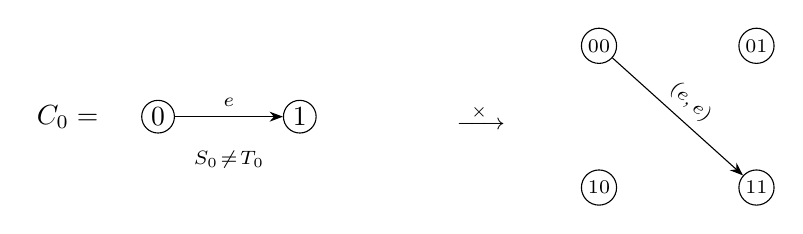
\begin{tikzpicture}[>=Stealth,baseline=(current bounding box.center)]
% C0 of Carr: loopless single edge 0 -> 1
  \node (lbl) at (-1.1,0) {$C_0=\;$};
  \node[circle,draw,inner sep=1.3pt] (a0) at (0,0) {$0$};
  \node[circle,draw,inner sep=1.3pt] (a1) at (1.8,0) {$1$};
  \draw[->] (a0) -- node[above,font=\scriptsize] {$e$} (a1);
  \node[font=\scriptsize] at (0.9,-0.55) {$S_0\!\neq\!T_0$};
% product (CxC)_0 = C0 x C0 : four vertices, ONE edge 00 -> 11 (pointwise product)
  \node[font=\footnotesize] at (4.1,0) {$\xrightarrow{\ \times\ }$};
  \node[circle,draw,inner sep=1.3pt] (00) at (5.6,0.9)  {\scriptsize $00$};
  \node[circle,draw,inner sep=1.3pt] (01) at (7.6,0.9)  {\scriptsize $01$};
  \node[circle,draw,inner sep=1.3pt] (10) at (5.6,-0.9) {\scriptsize $10$};
  \node[circle,draw,inner sep=1.3pt] (11) at (7.6,-0.9) {\scriptsize $11$};
  \draw[->] (00) -- node[sloped,above,font=\scriptsize] {$(e,e)$} (11);
\end{tikzpicture}
\caption{The acid-test witness $\mathtt{Carr}$: the object-of-objects graph $C_0=(0\xrightarrow{e}1)$
is loopless ($S_0\neq T_0$), hence has no global element $1\to C_0$. The product graph
$(C\times C)_0=C_0\times C_0$ is computed \emph{pointwise} in $\Graph$: four vertices and a single edge
$(e,e):00\to11$, again loopless (source $00\neq11$ target), so again no global element. The
identity-section and composition of $c\otimes c$ are nonetheless genuine graph morphisms --- the point
of the check.}
\label{fig:graph}
\end{figure}

We machine-check, in Lean~4 (core only, Mathlib-free), that for the three internal categories
$\mathtt{Cpt}$ (the point, a loop --- the negative control, \emph{with} a global element),
$\mathtt{Carr}$ ($C_0=(0\to1)$, loopless) and $\mathtt{Cdisc}$ ($C_0$ two loopless vertices), and all
nine ordered pairs, the Day tensor $c\otimes d$ computed fibrewise and glued by $S\times S,T\times T$
is a genuine internal category in $\Graph$: both fibres satisfy the category (= comonoid) axioms, and
the glued source/target are functors --- i.e. the identity-section and composition of $c\otimes d$
commute with $s,t$. The headline certificate is
\[
  \mathtt{all\_prod\_valid}:\ \mathtt{allProdValid}=\mathtt{true}
  \qquad(\text{by \texttt{decide}}),
\]
and the acid test is isolated as $\mathtt{prod\_st\_functors\_Carr\_Carr}$ together with
$\mathtt{prod\_loopless\_Carr\_Carr}$: for $\mathtt{Carr}\otimes\mathtt{Carr}$, whose
object-of-objects $(C\times C)_0$ (Figure~\ref{fig:graph}) is loopless and hence has no global element,
the source and target maps are nonetheless functors. Non-vacuity controls ($\mathtt{bogus}$ a
non-functor, $\mathtt{notcat}$ a non-category) are rejected by the same predicates. Every certificate
reports $\mathtt{[propext]}$ only --- no $\mathtt{sorryAx}$, no $\mathtt{native\_decide}$. This is, to
the author's knowledge, the first Lean certificate of a polynomial-comonoid computation internal to a
topos other than $\Set$. The $\Set$-side base case is checked independently by a Python verifier
($16/16$ ordered pairs over four test categories, on the nose).

%============================================================
\section{Discussion: honest bounds}\label{sec:discussion}
%============================================================

\subsection*{The maximal reach}
The argument needs the dependent sums $\Sigma$ that $\Poly(\Ee)$ à la Gambino--Kock requires. A bare
LCCC without the requisite coproducts is not covered; the honest maximal reach is ``any LCCC carrying
Gambino--Kock polynomials'', of which Grothendieck toposes are the canonical general-purpose case. We
have stated the theorems over Grothendieck toposes for that reason, and flag ``any such LCCC'' as the
open upper bound, decoupled from the main claim.

\subsection*{No converse packaged in}
We do \emph{not} assert a converse of the form ``LCCC $+$ extensive $\Rightarrow$ Grothendieck
topos''; the Giraud characterization of Grothendieck toposes is not of that shape, and we do not need
it. The theorems are stated directly over Grothendieck toposes, and \S\ref{sec:transport} records
which strictly weaker properties each line actually consumes.

\subsection*{Sheaf toposes come for free}
Because the proof uses only LCCC and finite-limit products --- both true in any Grothendieck topos,
sheaf or presheaf --- no separate left-exact-localization or sheafification step is required. The
earlier worry that sheaf toposes might need separate treatment dissolves: they are already covered by
the uniform statement.

\subsection*{What this buys the chain}
The equivalence $\text{containers}\simeq\cdots\simeq\Cat$ is now known to carry its monoidal content
--- product $=$ Day convolution $=$ Dirichlet tensor --- uniformly across every Grothendieck topos. A
compositional model built in presheaves on a site, or sheaves on a space, inherits the product
structure of its directed shapes with no recomputation and no appeal to global elements. That the
construction wants precisely a locally cartesian closed home, and finds one in every topos, is the
stable form of the ``which base?'' question the program began with.

%============================================================
\begin{thebibliography}{9}

\bibitem{GambinoKock2013}
N.~Gambino and J.~Kock,
\emph{Polynomial functors and polynomial monads},
Math. Proc. Cambridge Philos. Soc. \textbf{154} (2013), no.~1, 153--192; arXiv:0906.4931.

\bibitem{LucyshynWright2025}
R.~B.~B.~Lucyshyn-Wright,
\emph{$\mathcal{V}$-graded categories and $\mathcal{V}$-$\mathcal{W}$-bigraded categories}, 2025;
arXiv:2502.18557.

\bibitem{NiuSpivak2023}
N.~Niu and D.~I.~Spivak,
\emph{Polynomial Functors: A Mathematical Theory of Interaction}, book draft, 2023; arXiv:2312.00990.

\bibitem{ShapiroSpivak2023}
B.~Shapiro and D.~I.~Spivak,
\emph{Structures on Categories of Polynomials}, 2023; arXiv:2305.00167.

\bibitem{SGF2021}
D.~I.~Spivak, R.~Garner, and A.~Fairbanks(-Lyons),
\emph{Functorial Aggregation}, 2021; arXiv:2111.10968.

\end{thebibliography}

\end{document}
